obdelava%******************************* UVOD ******************************************
\chapter{Uvod} \label{uvod}

Digitalna vezja uporabljamo za obdelavo podatkov. Z njimi implementiramo algoritme, ki iščejo praštevila, rešujejo enačbe itd.

Teoretično lahko poljuben algoritem implementiramo z ogromno tabelo. Glede na vhodne podatke preprosto najdemo pripadajočo rešitev. Prednost takega pristopa je, da ne potrebujemo nikakršnega spomina. Takšnim vezjem pravimo \textbf{kombinatorična vezja}. Kombinatorična vezja so pogosto uporabljena za osnovne operacije npr. logične funkcije(IN, ALI...), seštevanje, primerjava števil itd. ne pa za implementacijo celotnih algoritmov.

\begin{figure}[H]
	\centering
	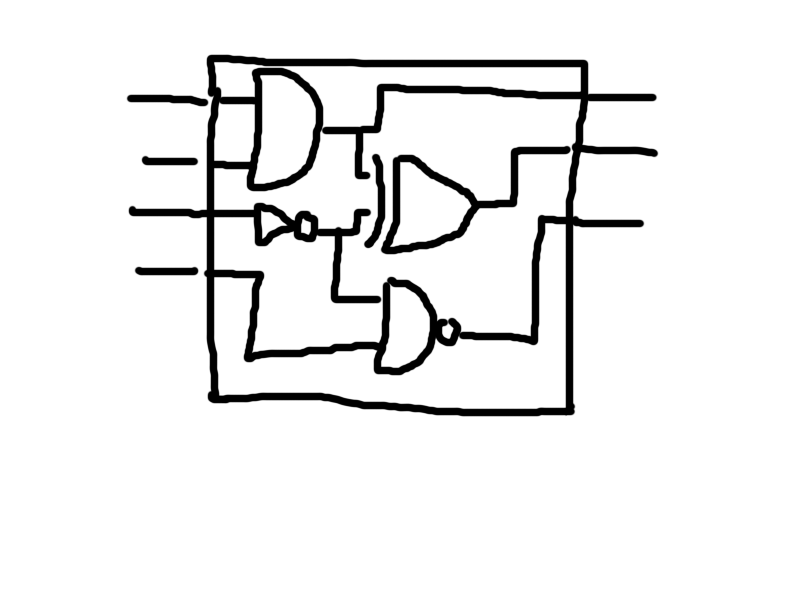
\includegraphics[width=0.7\linewidth]{slike/uvod/comb}
	\caption{}
	\label{fig:comb}
\end{figure}


Problem kombinatoričnih vezji je \textbf{skaliranje}. Ko raste število vhodov in izhodov rastejo tudi površina, ki jo vezje porabi in čas, ki ga vezje porabi, da izračuna rezultat. 
Površina raste proporcionalno številu vhodov.
Zakasnitev raste proporcionalno kvadratu številu vhodov.
Iz teh razlogov, želimo omejiti velikost posameznih kombinatoričnih vezji.

Rešitev je, da uporabimo iterativne algoritme. Torej obdelujemo podatke v manjših kosih. To omeji velikost potrebnih kombinatoričnih vezji in dovoli večkratno uporabo istih kombinatoričnih vezji. To zahteva, da izhod kombinatoričnega vezja povežemo nazaj na vhod oz., da naredimo povratno vezavo. Izhod takih vezji ni več odvisen le od vhodov, temveč tudi od stanja povratne zanke, torej imajo taka vezja spomin, imenujejo se \textbf{sekvenčna vezja}.

\begin{figure}[H]
	\centering
	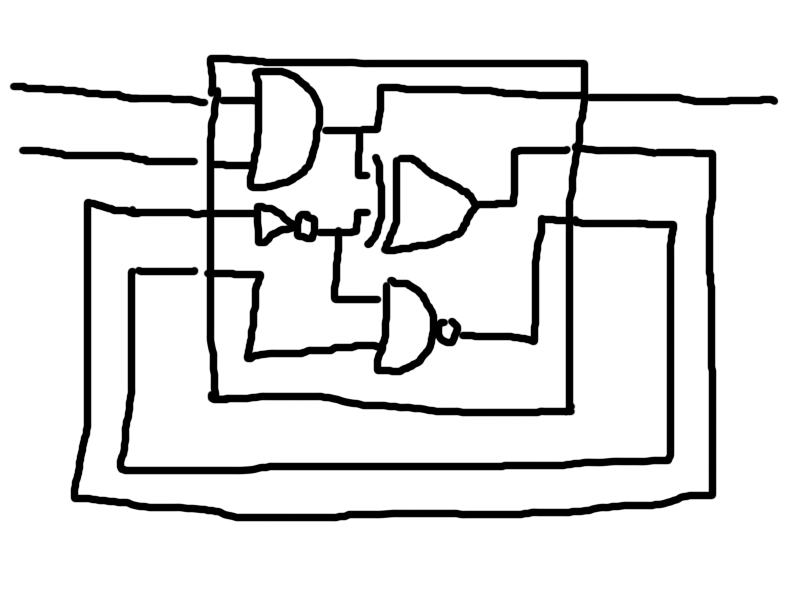
\includegraphics[width=0.7\linewidth]{slike/uvod/comb_fb}
	\caption{}
	\label{fig:comb}
\end{figure}


Ampak tu se pojavi nova težava. Predstavljajmo si seštevalnik, katerega izhod povežemo na enega izmed vhodov, na drugi vhod postavimo konstanto 1.
Želeli bi si, da vezje šteje 1,2,3... Ampak to se ne zgodi, namesto tega na izhodu dobimo kaotične signale. Razlog je, da je v vezju ogromno število povratnih zank, vendar med seboj niso sinhronizirane. Vsaka povratna zanka ima rahlo drugačno zakasnitev, zato zanke počasi zlezejo iz faze. Rezultat je, da vezje ni stabilno in ne opravlja želene naloge. 

Nujno je torej vpeljati mehanizem s katerim periodično sinhroniziramo vse povratne zanke. To storimo s spominskimi elementi, ki jih vstavimo v povratno vezavo, imenujemo jih \textbf{registri}. Registri shranijo podatke na svojem vhodu in jih oddajo na izhodu. Njihova naloga je, da ne prepustijo naprej novih podatkov, dokler niso stari podatki ponovno obdelani. Efektivno ponovno sinhronizirajo faze vseh povratnih zank.

Torej moramo izvedeti kdaj so podatki na vhodu registra obdelani. Takrat lahko register sprejme nove podatke. Podatki so obdelani, ko se spropagirajo skozi \textbf{najdaljšo} izmed vseh povratnih zank.

V splošnem imamo dva načina na katera lahko storimo:


\begin{itemize}
	\item Globalna sinhronizacija(Taktni signal):
	V tej shemi uporabimo predpostavko, da obdelava podatkov v \textbf{vseh} vezjih med dvema zaporednima registroma ne traja dlje od neke konstante. Vse registre nato naenkrat sprožimo z to periodo. To storimo s taktnim signalom.	 \footnote{Taktni signal je ustvarjen prek kristalnega oscilatorja ali RC oscilatorja. Vse povratne zanke v vezju nato sinhronizirano z tem oscilatorjem, ki mora imeti najdaljšo periodo.}
	\begin{figure}[H]
		\centering
		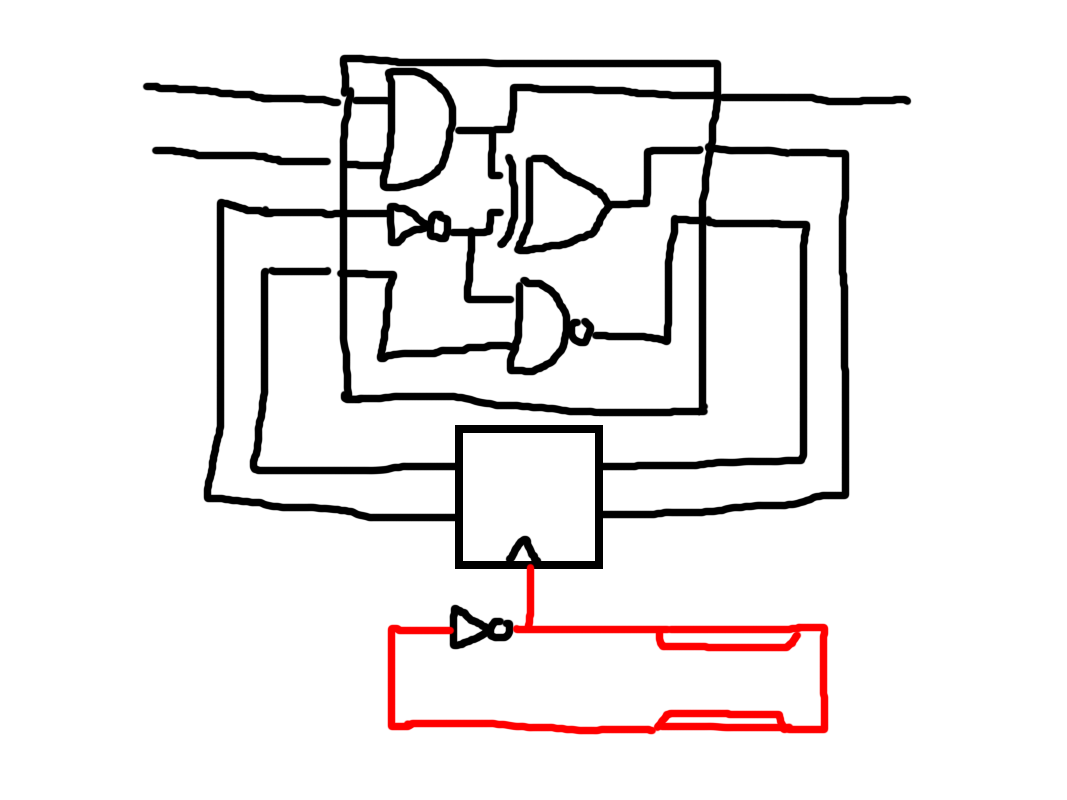
\includegraphics[width=0.7\linewidth]{slike/uvod/seq}
		\caption{}
		\label{fig:comb}
	\end{figure}
	
	
	
	
	\item Lokalna sinhronizacija:
	V tej shemi sinhroniziramo vse povratne zanke na \textbf{najdaljšo} izmed povratnih zank. Vezje moramo zasnovati tako, da je ta zanka vedno najdaljša, neodvisno od variacij v vezju in vhodnih podatkih.
	
	\begin{figure}[H]
		\centering
		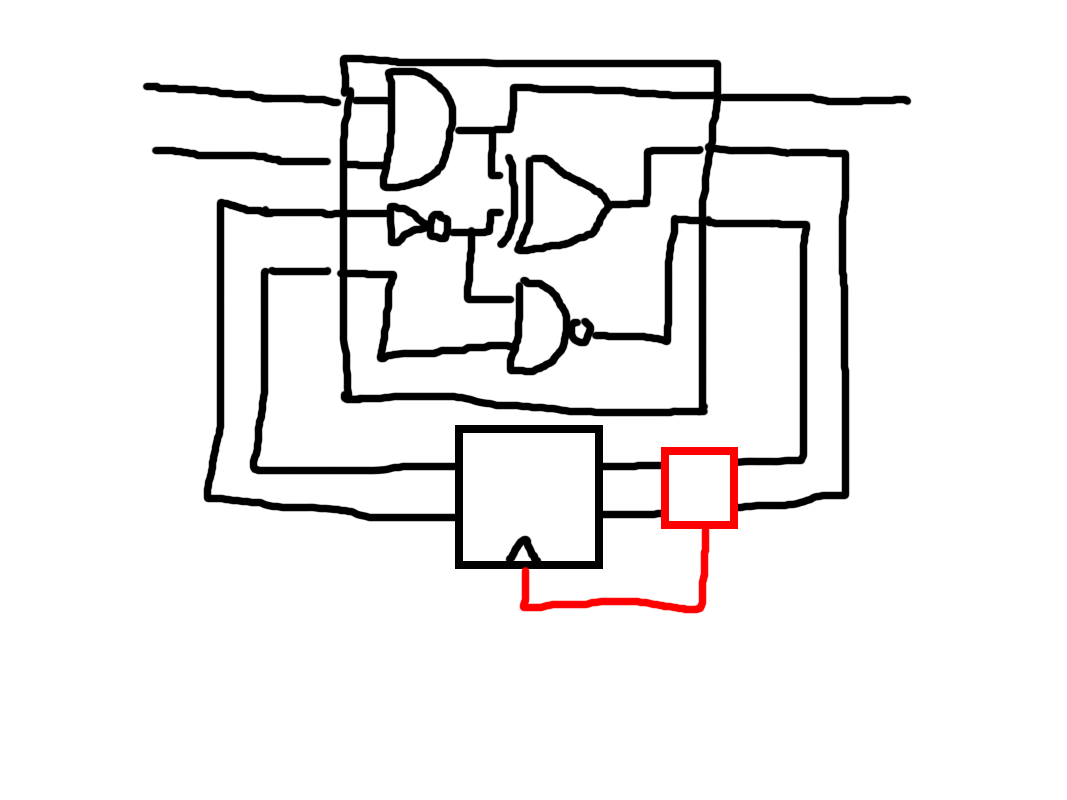
\includegraphics[width=0.7\linewidth]{slike/uvod/async}
		\caption{}
		\label{fig:comb}
	\end{figure}
	
\end{itemize}


	

	

	





	
